\documentclass[11pt,oneside]{article}
\input{coursHeadings}
\usepackage[raccourcis]{FAST}
\usepackage[%
    pdftitle={Produits Procédés Matériaux -- },
    pdfauthor={Xavier Pessoles},
    colorlinks=true,
    linkcolor=blue,
    citecolor=magenta]{hyperref}
\usepackage{schemabloc}



% \makeatletter \let\ps@plain\ps@empty \makeatother
%% DEBUT DU DOCUMENT
%% =================
\sloppy
\hyphenpenalty 10000

\newcommand{\Pointilles}[1][3]{%
\multido{}{#1}{\makebox[\linewidth]{\dotfill}\\[\parskip]
}}


\colorlet{shadecolor}{orange!15}

\newtheorem{theorem}{Theorem}


\begin{document}


\newboolean{prof}
\setboolean{prof}{true}
%------------- En tetes et Pieds de Pages ------------
\pagestyle{fancy}
\renewcommand{\headrulewidth}{0pt}

\fancyhead{}
\fancyhead[L]{%
\noindent\noindent\begin{minipage}[c]{2.6cm}
%Lycée Rouvière PTSI
\includegraphics[width=2cm]{png/logo_ptsi.png}%
\end{minipage}
}

\fancyhead[C]{\rule{12cm}{.5pt}}

\fancyhead[R]{%
\noindent\begin{minipage}[c]{3cm}
\begin{flushright}
\footnotesize{\textit{\textsf{Sciences Industrielles\\ pour l'Ingénieur}}}%
\end{flushright}
\end{minipage}
}

\renewcommand{\footrulewidth}{0.2pt}

\fancyfoot[C]{\footnotesize{\bfseries \thepage}}
\fancyfoot[L]{\footnotesize{2012 -- 2013} \\ X. \textsc{Pessoles}}
\ifthenelse{\boolean{prof}}{%
\fancyfoot[R]{\footnotesize{Cours -- CI 6 : PPM -- P}}
}{%
\fancyfoot[R]{\footnotesize{Cours -- CI 6 : PPM}}
}



\begin{center}
 \huge\textsc{CI 6 -- PPM -- Produits Procédés Matériaux}

 \large\textsc{Élaboration des pièces mécaniques. Introduction de la chaîne numérique}
\end{center}

\begin{center}
 \LARGE\textsc{Chapitre 1 -- Introduction aux matériaux}
\end{center}

\vspace{.5cm}

\begin{center}
\begin{tabular}{cccc}
\includegraphics[height=2.5cm]{png/acier} &
\includegraphics[height=2.5cm]{png/bois} &
\includegraphics[height=2.5cm]{png/composite} &
\includegraphics[height=2.5cm]{png/verre}\\
\textit{Acier \cite{acier}} & 
\textit{Bois} & 
\textit{Fibre de carbone \cite{composite}} & 
\textit{Verre \cite{verre}} \\
\end{tabular}
\end{center}

Tous les objets que nous rencontrons sont faits de matière. Suivant les fonctions que doit réaliser cet objet, des choix ont dû être fait pour faire le choix des matériaux qui le constituent. Parmi la multitude de matériaux existants (matériaux métalliques, plastiques, composites, organiques ...) nous allons nous demander quels sont les critères qui ont poussé au choix d'un matériau. Le but de ce cours est donc de présenter les familles de matériaux ainsi quel leur caractéristiques. Il doit aussi permettre de décrire les essais permettant de déterminer les caractéristiques mécaniques de matériaux.



\begin{prob}
\textsc{Problématique :}

En phase d'avant conception d'un produit, quels sont les critères qui vont permettre de choisir les matériaux à utiliser ?
\end{prob}

\begin{savoir}
\textsc{Savoirs :}
\begin{itemize}
\item Classifier les différents matériaux et leurs principales caractéristiques
%\item Classifier et désigner un matériau métallique.
%\item Donner les propriétés d'un matériau métallique.
%\item Analyser les essais provenant d'un essai mécanique. 
\end{itemize}
\end{savoir}

%\newpage 

\setlength{\parskip}{0ex plus 0.2ex minus 0ex}
 \renewcommand{\contentsname}{}
 \renewcommand{\baselinestretch}{1}

\tableofcontents

 \renewcommand{\baselinestretch}{1.2}
\setlength{\parskip}{2ex plus 0.5ex minus 0.2ex}

% \vspace{1cm}
\textit{Ce document est en évolution permanente. Merci de signaler toutes
erreurs ou coquilles.}

%\newpage

\section{Généralités sur les matériaux}
\subsection{Propriétés des matériaux}
Le choix d'un matériau va se faire à partir des \textbf{fonctions} que doit réaliser un produit. 
Si le produit doit répondre à des fonctions esthétiques, on lui demandera par exemple de pouvoir se mettre en forme facilement ou de pouvoir être teinté. Si le produit doit transmettre une puissance mécanique élevée, on lui demandera d'être résistant à des actions mécaniques. Si le
produit doit être au contact d'une source de chaleur, on lui demandera d'avoir un point de fusion élevé ...

De plus, un même produit devant répondre à un grand nombre de fonctions, les contraintes vont alors se multiplier.

Ainsi, parmi les critères de choix d'un matériau on peut citer les suivants :
\begin{itemize}
\item critères mécaniques :
\begin{itemize}
\item être léger;
\item résister aux chocs;
\item résister aux efforts de traction/compression;
\item résister à une sollicitation en fatigue;
\end{itemize}
\item critères chimiques :
\begin{itemize}
\item résister à la corrosion;
\item être biodégradable;
\item ne pas agresser l'environnement
\end{itemize}
\item critères électriques :
\begin{itemize}
\item être isolants ou conducteurs d'électricité;
\end{itemize}
\item critères physiques :
\begin{itemize}
\item être magnétique ou non;
\item avoir une température de fusion donnée;
\item conduire la chaleur;
\item limiter les dilatations thermiques;
\end{itemize}
\item critères de mise en forme :
\begin{itemize}
\item coulabilité; 
\item usinabilité; 
\item soudabilité; 
\end{itemize}
\item critère économique :
\begin{itemize}
\item être le moins cher possible...
\end{itemize}
\end{itemize}

Un matériau est donc à choisir en fonction de tous ces critères. 

\subsection{Familles de matériaux}

Les matériaux peuvent être classifiés en différentes familles. 

\begin{minipage}[c]{.6\linewidth}
Tout d'abord les matériaux métalliques ont, en général, la particularité d'être opaques, solides, denses, bons conducteurs de chaleur et d'électricité et d'avoir une plasticité qui permet de les déformer. Parmi les matériaux métalliques, on distingue les métaux ferreux (aciers et fontes) et les matériaux non ferreux (alliages de cuivre, d'aluminium, de magnésium, de titane ...).
\end{minipage} \hfill
\begin{minipage}[c]{.35\linewidth}
\begin{center}
\begin{tabular}{cc}
\includegraphics[height=1.5cm]{png/mobidisc1}&
\includegraphics[height=1.5cm]{png/mobidisc2}
\\
\end{tabular}
\textit{Prothèse de disque lombaire -- Acier allié (Chrome Cobalt) \cite{ldr}}
\end{center}
\end{minipage}

\vspace{.5cm}

Les matériaux polymères, ont la particularité d'être peu denses, de bons isolants et à être facile à mettre en \oe{}uvre. Il existe des polymères d'origine végétale (comme le bois ou le papier) et des polymères synthétiques, provenant de l'industrie chimique et pétrolière. Parmi les polymères synthétiques on distingue en général les thermoplastiques, les thermodurcissables et les élastomères. 


\begin{minipage}[c]{.3\linewidth}
\begin{center}
\begin{tabular}{c}
\includegraphics[height=2cm]{png/dent}
\\
\end{tabular}

\textit{Prothèse de dent en céramique \cite{dent}}
\end{center}
\end{minipage}\hfill
\begin{minipage}[c]{.65\linewidth}
Les matériaux céramiques ont une grande rigidité, une résistance thermique élevée, sont dures mais fragiles et difficiles à former. On distingue les céramiques traditionnelles (ciment, argile, plâtre ...) et les céramiques techniques.
\end{minipage}

\vspace{.5cm}

Les matériaux composites permettent d'avoir des caractéristiques supérieures à des matériaux simples. Ils peuvent être plus légers, plus rigides mais il peut être assez difficile de les mettre en forme. Ils sont composés de deux matériaux non miscibles appelés matrice et renfort. 

\begin{minipage}[c]{.3\linewidth}
\begin{center}
\begin{tabular}{c}
\includegraphics[height=2cm]{png/wafer}
\\
\end{tabular}

\textit{Wafer de Silicium \cite{wafer} -- C\oe{}urs de processeurs}
\end{center}
\end{minipage}\hfill
\begin{minipage}[c]{.65\linewidth}
Enfin, d'autres matériaux comme les semi conducteurs possèdent des caractéristiques électriques qui leur permettent de trouver de nombreuses applications industrielles. 
\end{minipage}

\vspace{.5cm}


\subsection{Structure cristalline des matériaux métalliques}
Les métaux sont formés de cristaux, c'est-à-dire de mailles élémentaires qui se répètent suivant les 3 directions de l'espace. On peut rencontrer les organisations cristallines suivantes : 

\noindent
\begin{minipage}[c]{.3\linewidth}
\begin{center}
\includegraphics[height=1.5cm]{png/cfc}

\textit{Maille cubique face centrée}
\end{center}
\end{minipage}
\hfill
\begin{minipage}[c]{.3\linewidth}
\begin{center}
\includegraphics[height=1.5cm]{png/cc}

\textit{Maille cubique centrée}
\end{center}
\end{minipage}
\hfill
\begin{minipage}[c]{.3\linewidth}
\begin{center}
\includegraphics[height=1.5cm]{png/hc}

\textit{Maille hexagonale compacte}
\end{center}
\end{minipage}

La structure cristalline des matériaux va changer leur propriété physique. Ainsi un même matériau n'aura pas les mêmes caractéristiques suivant sa structure cristalline. Par exemple, le diamant et le graphite sont tous les deux composés de carbone. Cependant, l'organisation des atomes de carbone n'est pas la même pour ces 2 matériaux. 

\begin{exemple}
Le fer pur sous sa forme $\alpha$ est structuré en CC (cubique centré, paramètre de maille 0,2866 $nm$). Le fer $\gamma$ (qui apparaît a une température de $916^\text{o}C$ est structuré en CFC (cubique face centrée, paramètre de maille 0,3647 $nm$.
\end{exemple}


Les métaux utilisés sont, la plupart du temps, des alliages de plusieurs composants. Dans les mailles définies précédemment, il existe des écarts entre chacune des sphères. Ces écarts sont appelés sites intersticiels. Lorsque dans un alliage un atome et beaucoup plus petit que l'autre, il peut être amené à loger dans ces sites intersticiels.

Dans d'autres cas, les alliages vont conserver une structure cristalline définie. Cependant, les atomes de la maille ne seront pas les mêmes. On parle de solution solide de substitution. 



\section{Les familles de matériaux}
\subsection{Les fontes et les aciers}
\begin{defi}

Les fontes et les aciers sont des alliages de fer et de carbone auxquels on peut adjoindre des éléments d'addition. 

Dans l'acier, le pourcentage de carbone est compris entre 0,008 et 2,11\%. 

Dans la fonte, le pourcentage de carbone est compris entre 2,11 et 6,67\%. 

\end{defi}


En construction mécanique, les fontes sont principalement utilisées lorsque d'une part il n'existe ni contrainte mécanique élevée ni contrainte de poids. Et que, d'autre part, la géométrie de la pièce demande à ce qu'elle soit réalisée en fonderie.

De manière générale, les aciers sont utilisés lorsque les produits conçus sont sollicités mécaniquements. 

\begin{minipage}[c]{.45\linewidth}
\begin{center}
\includegraphics[height=3cm]{png/carter}

\textit{Carter de réducteur roue-vis en fonte (moulé) \cite{carter}}
\end{center}
\end{minipage}\hfill
\begin{minipage}[c]{.45\linewidth}
\begin{center}
\includegraphics[height=3cm]{png/bielles}

\textit{Bielles en acier (forgées)}
\end{center}
\end{minipage}


\subsubsection{Obtention des fontes et des aciers}
Les matériaux ferreux sont obtenus à partitr d'oxyde de fer associé à de la terre et de la roche (gangue). Le minerai de fer doit contenir plus de 30\% de fer pour être éconiquement exploitable.
La première opération consiste en une séparation de la terre et de la roche du reste du minerai dans le but d'obtenir un minerai enrichi. 

Ce minerai enrichi est associé à du coke (dérivé de la houille et composé essentiellement de carbone) dans de hauts fourneaux. L'élévation de la température est obtenue grâce à la combustion du coke. A l'état liquide, la fonte se sépare du laitier (constitué de la gangue) par gravitation. 

Suivant la quantité de coke, on obtient de la fonte \textbf{blanche} ou de la {fonte grise de première fusion}.


\paragraph{Obtention de la fonte}
Suivant la forme du graphite dans la matrice de fer, il est possible d'obtenir plusieurs types de fonte : 

\begin{itemize}
\item les fontes à graphite lamellaires sont obtenues par chauffage et décarburation de la fonte grise;
\item les fontes à graphite sphéroïdal sont obtenues par chauffage, décarburation et traitement au magnésium et silicium de la fonte grise;
\item les fontes à graphite nodulaire sont obtenues par un chauffage long (10 heures à $950^{\text{o}}C$) dans un milieu neutre ou en présence d'oxygène puis par un refroidissement à vitesse variable. 
\end{itemize}

\paragraph{Obtention de l'acier}

Pour obtenir de l'acier, il est nécessaire de décarburer le fonte. Pour cela, la fonte (blanche) est fondue dans des fours ou par des arcs électriques. Dans le cas des fours, la décarburation est réalisée par une insufflation d'air enrichi en oxygène. 

\subsubsection{Le diagramme Fer -- Carbone}
Nous avons vu que l'acier et la fonte sont des alliages de fer et de carbone. Ainsi, suivant la concentration de carbone et la température, la structure de l'alliage peut changer. 

La diagramme fer--carbone ci-dessous permet de mettre en valeur les différents états existants. 
\begin{center}
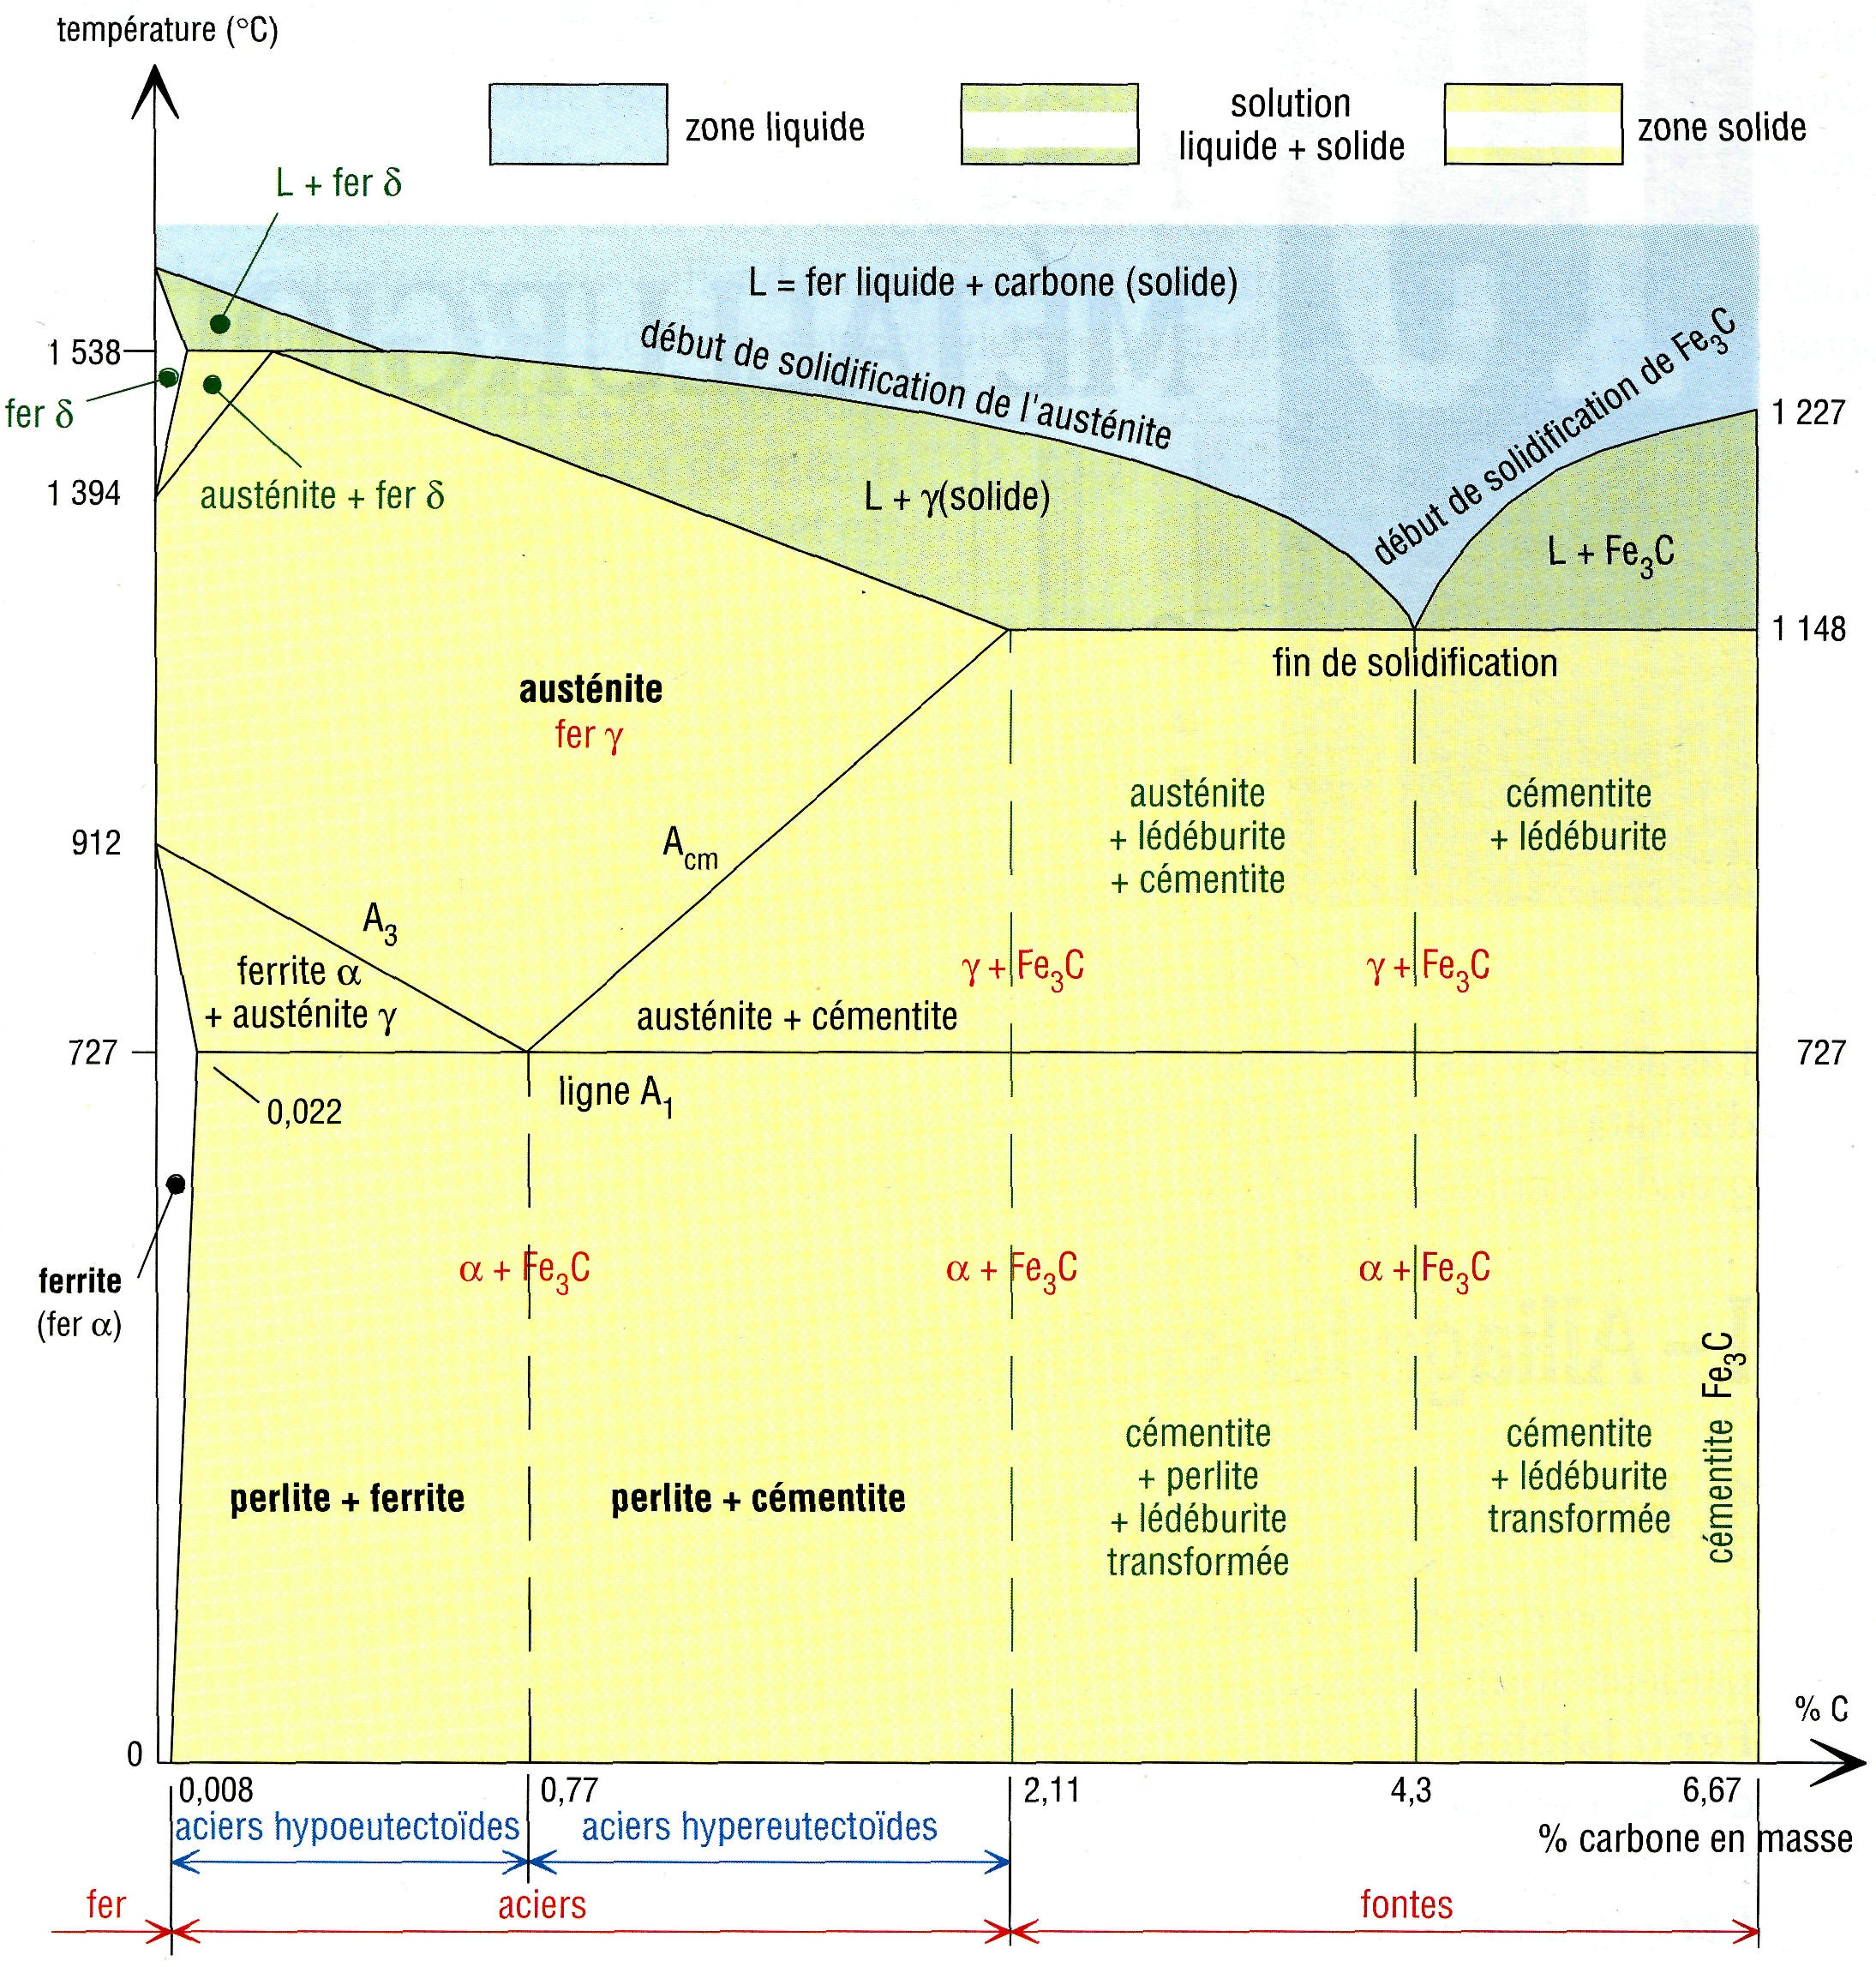
\includegraphics[width=.8\textwidth]{png/FerCarbone}

\textit{Diagarmme fer -- carbone \cite{fer}}
\end{center}

Le fer $\alpha$ se trouve pour des températures inférieures à $912^\text{o}C$. Le cristal est de type cubique face centré. Lorsque du carbone est inséré dans la maille de fer $\alpha$, le composé est appelé ferrite. 

La cémentite, de composition chimiqie $Fe_3 C$ est aussi appelé carbure de fer. Elle est rencontrée à l'état pur dans la fonte titrant à 6,67\% de carbone. Ce composé est très dur et très cassant. Il est très rarement utilisé. 

La perlite est composé de ferrite et de cémentite. Elle titre à 0,85\% de carbone. 

A haute température, on trouve du fer $\gamma$, dont le cristal est de type cubique face centrée. De par sa structure, il est donc plus dense que le fer $\alpha$. Lorsque des atomes de carbone viennent se loger dans les sites intersticiels on parle alors d'austénite. 

\subsection{Les alliages d'aluminium}

Les alliages d'aluminium sont utilisés d'une part pour leur faible poids. En effet, l'aluminium a une densité de 2,7 (contre 7,5 à 8,1 pour l'acier et 6,8 à 7,4 pour la fonte). Il a par ailleurs une très bonne tenue à la corrosion. En effet, en présence d'oxygène, une couche d'alumine recouvre l'aluminium. Cette couche étanche protège le c\oe{}ur du matériau. 

Par ailleurs, l'aluminium a la particularité de très bien conduire l'électricité et d'être amagnétique. 

Enfin, sa malléabilité et sa coulabilité lui permettent dêtre emboutis et moulés aisément. 

En revanche, les caractéristiques mécaniques telles que la dureté ou le module d'élasticité sont plus faibles que pour les aciers.

\subsection{Les alliages de cuivre}
Le cuivre a la principale caractéristique d'être un très bon conducteur. Il est donc utilisé pour conduire l'électricité (fils électriques des installations domestiques, bobinage de moteurs ...) ou pour conduire la chaleur (casseroles de nos grands-mères). 

Il offre par ailleurs une très bonne résistance à la corrosion (d'où son utilisation dans les toitures).

L'ajout d'éléments d'addition comme l'étain (donnant ainsi du bronze) lui permet d'avoir des coefficients de frottement amoindris. Lorsqu'il est allié avec du zinc (laiton), le cuivre est très utilisé en plomberie. 

\begin{minipage}[c]{.3\linewidth}
\begin{center}
\includegraphics[height=3cm]{png/casserole}

\textit{Casseroles en cuivre}
\end{center}
\end{minipage}\hfill
\begin{minipage}[c]{.3\linewidth}
\begin{center}
\includegraphics[height=3cm]{png/coussinets}

\textit{Paliers lisses}
\end{center}
\end{minipage}\hfill
\begin{minipage}[c]{.3\linewidth}
\begin{center}
\includegraphics[height=3cm]{png/raccord}

\textit{Raccord de plomberie}
\end{center}
\end{minipage}

\subsection{Les matériaux composites}

Les matériaux composites sont composés d'une matrice et d'un renfort. On rencontre aussi bien des matériaux naturels qu'artificiels : 

\begin{itemize}
\item le bois est constitué d'une matrice de lignine et de renforts en fibre de cellulose;
\item le béton armé est constitué d'une matrice en béton et de renforts en acier;
\item les matériaux composites utilisés dans l'aéronautique sont constitués d'une matrice époxy avec des renforts en fibre de carbone;
\item les matériaux composites utilisés dans le milieu nautique (loisir) sont constitués d'une matrice époxy avec des renforts en fibre de verre...
\end{itemize}

Plusieurs procédés permettent de mettre en forme les matériaux composites. On peut par exemple citer le moulage par contact qui permet de fabriquer des coques diverses (coques de bateau, voilure d'avions ...). Dans le cadre de ce procédé, lorsque le renfort est préimprégné avec de la résine :

\begin{minipage}[c]{.6\linewidth}
\begin{itemize}
\item il est d'abord nécessaire de fabriquer un moule;
\item le moule est enduit avec un produit favorisant le démoulage de la pièce;
\item le moule est ensuite recouvert avec des couches de fibre préimprégnée. Dans le but d'obtenir des performances identiques dans chaque direction, les couches sont souvent croisées;
\item l'ensemble est mis sous vide dans le but se débarrasser des bulles d'air; 
\item l'ensemble est alors polymérisé dans un four (autoclave);
\item la pièce est démoulée puis détourée. 
\end{itemize}
\end{minipage}\hfill
\begin{minipage}[c]{.35\linewidth}
\begin{center}
\includegraphics[width=.9\textwidth]{png/a350}

\textit{Drapage de l'aile de l'A350 \cite{a350}}
\end{center}
\end{minipage}

\vspace{.5cm}

Ces matériaux ont la particularité d'avoir de bonnes caractéristiques mécaniques pour une densité relativement faible. Ils ont aussi une bonne résistance à la fatigue. Ils ont cependant une mauvaise résistance aux impacts. Le perçage et l'usinage de ces matériaux peut aussi poser de nombreux problèmes.

\subsection{Les céramiques}

Historiquement, les céramiques étaient les matériaux fabriqués à partir de terre cuite. Les céramiques utilisées en conception mécanique sont appelées céramiques techniques. 

Elles ont comme propriété d'avoir une grande résistance mécanique, une dureté élevée ainsi qu'une grande résistance à l'usure. Ces propriétés sont conservées à haute température. Elles ont aussi la propriété d'être isolantes. En revanche, les céramiques résistent peu à des chocs mécaniques. 

Par ailleurs, étant neutres et amorphes, elles sont sans danger pour l'homme et pour l'environnement ce qui leur permet d'être utilisés dans le biomédical. 


Les céramiques sont composées de deux oxydes. Ceux-ci sont réduits à l'état de poudre puis mélangés à haute température (en dessous du point de fusion). Les poudres vont alors s'agréger par diffusion. 


\begin{thebibliography}{2}
\bibitem{acier}{\url{http://www.lefigaro.fr/medias/2008/12/18/47e0e366-cd2c-11dd-882f-4b99bc2f9b71.jpg}}
\bibitem{composite}{\url{http://fr.gurit.com/benefits-of-composite-materials.aspx}}
\bibitem{verre}{\url{http://www.vezenobres.info/partenaires.htm}}
\bibitem{ldr}{LDR Médical \url{http://fr.ldrmedical.com/Produits/Thoraco-lombaire/MobidiscProthèsededisquelombaire}}
\bibitem{dent}{Protilab \url{http://www.protilab.com/fr/prothese/7/Couronne+sur+implant}}
\bibitem{wafer}{\url{http://www.efficacite-electrique.fr/2012/03/usa-semi-conducteurs-plus-compacts-meilleure-efficacite-electrique/}}
\bibitem{carter}{\url{http://www.directindustry.fr/prod/sermes/moto-reducteurs-electriques-a-vis-sans-fin-a-carter-en-fonte-7542-424078.html}}
\bibitem{fer}{\url{http://www.zpag.net/Tecnologies_Indistrielles/Metaux_Ferreux.htm}}
\bibitem{a350}{© Airbus S.A.S.}

\bibitem{rb}{Supports de cours de Renan Bonnard,PTSI, Lycée Newton, Clichy la Garenne}
\bibitem{jb}{Supports de cours de Joël Boiron, PTSI, Lycée Gustave Eiffel, Bordeaux}
%\bibitem{wikipedia}{Wikipédia, Dureté (matériau) --- Wikipédia{,} l'encyclopédie libre, 2012, \url{
%http://fr.wikipedia.org/w/index.php?title=Duret\%C3\%A9_(mat\%C3\%A9riau)\&oldid=83575804}}
%\bibitem{mc}{Supports de cours de Maryline Carrez, Lycée Jules Haag, Besançon}
%\bibitem{pf}{Supports de cours de Philippe Fichou, Lycée Vauban, Brest \url{http://philippe.fichou.pagesperso-orange.fr/documents/liaisoncomplete2003.pdf}}
%\bibitem{jpp}{Supports de cours de Jean-Pierre Pupier, Lycée Rouvière, Toulon}

\end{thebibliography}

\end{document}